\section{Formal Languages and Automata}
Pattern matching is central to many applications and supported by regular expressions in programming languages. The Chomsky hierarchy of Formal Languages provides a theory of programming languages of increasing expressively. Formal Automata or Machines are models of computation, that implement languages of the Chomsky hierarchy.
\subsection{Regular Expressions}
A regular expression describes a pattern, it has very basic operators however with these operations it can specify a usually infinite set of strings see table \ref{tab:regex}. \footnote{RegExp cheat sheet \href{https://www.cheatography.com/davechild/cheat-sheets/regular-expressions/}{(link)}}
\begin{table}[h]
\begin{tabular}{llll}
\hline
\multicolumn{1}{|l|}{\textbf{Operation}} & \multicolumn{1}{l|}{\textbf{Regular Expression}} & \multicolumn{1}{l|}{\textbf{Yes}} & \multicolumn{1}{l|}{\textbf{No}} \\ \hline
\multicolumn{1}{|l|}{Concatenation} & \multicolumn{1}{l|}{aabbaab} & \multicolumn{1}{l|}{aabaab} & \multicolumn{1}{l|}{Every Other String} \\ \hline
\multicolumn{1}{|l|}{Wildcard} & \multicolumn{1}{l|}{.u.u.u.} & \multicolumn{1}{l|}{\begin{tabular}[c]{@{}l@{}}cumulus\\ jugulum\end{tabular}} & \multicolumn{1}{l|}{\begin{tabular}[c]{@{}l@{}}succubus\\ tumultuous\end{tabular}} \\ \hline
\multicolumn{1}{|l|}{Union} & \multicolumn{1}{l|}{aa | baab} & \multicolumn{1}{l|}{\begin{tabular}[c]{@{}l@{}}aa\\ babb\end{tabular}} & \multicolumn{1}{l|}{Every Other String} \\ \hline
\multicolumn{1}{|l|}{Closure} & \multicolumn{1}{l|}{ab*a} & \multicolumn{1}{l|}{\begin{tabular}[c]{@{}l@{}}aa\\ abbba\end{tabular}} & \multicolumn{1}{l|}{\begin{tabular}[c]{@{}l@{}}ab\\ ababa\end{tabular}} \\ \hline
\multicolumn{1}{|l|}{\multirow{2}{*}{Parentheses}} & \multicolumn{1}{l|}{a(a|b)aab} & \multicolumn{1}{l|}{\begin{tabular}[c]{@{}l@{}}aaaab\\ abaab\end{tabular}} & \multicolumn{1}{l|}{Every Other String} \\ \cline{2-4} 
\multicolumn{1}{|l|}{} & \multicolumn{1}{l|}{(ab)*a} & \multicolumn{1}{l|}{\begin{tabular}[c]{@{}l@{}}a\\ ababababa\end{tabular}} & \multicolumn{1}{l|}{\begin{tabular}[c]{@{}l@{}}\varepsilon\\ abbbaa\end{tabular}} \\ \hline
\end{tabular}
\caption{Regex}
\label{tab:regex}
\end{table}
\subsubsection{Generalised Regular Expressions}
These have all of the rules previously mentioned however they also have more as seen in the table \ref{tab:Gregex}
\begin{table}[H]
\begin{tabular}{llll}
\hline
\multicolumn{1}{|l|}{\textbf{Operation}} & \multicolumn{1}{l|}{\textbf{Regular Expression}} & \multicolumn{1}{l|}{\textbf{Yes}} & \multicolumn{1}{l|}{\textbf{No}} \\ \hline
\multicolumn{1}{|l|}{One or more} & \multicolumn{1}{l|}{a(bc)+de} & \multicolumn{1}{l|}{\begin{tabular}[c]{@{}l@{}}abcde\\ abcbcde\end{tabular}} & \multicolumn{1}{l|}{\begin{tabular}[c]{@{}l@{}}ade\\ bcde\end{tabular}} \\ \hline
\multicolumn{1}{|l|}{Character classes} & \multicolumn{1}{l|}{{[}A-Za-z{]}{[}a-z{]}*} & \multicolumn{1}{l|}{\begin{tabular}[c]{@{}l@{}}capitalised\\ Word\end{tabular}} & \multicolumn{1}{l|}{\begin{tabular}[c]{@{}l@{}}camelCase\\ 4illegal\end{tabular}} \\ \hline
\multicolumn{1}{|l|}{Exactly k} & \multicolumn{1}{l|}{{[}0-9{]}\{5\}-{[}0-9{]}\{4\}} & \multicolumn{1}{l|}{\begin{tabular}[c]{@{}l@{}}08540-1321\\ 19072-5541\end{tabular}} & \multicolumn{1}{l|}{\begin{tabular}[c]{@{}l@{}}111111111111\\ 166-54-111\end{tabular}} \\ \hline
\multicolumn{1}{|l|}{Negations} & \multicolumn{1}{l|}{{[}\textasciicircum{}aeiob{]}\{6\}} & \multicolumn{1}{l|}{rhythm} & \multicolumn{1}{l|}{decade} \\ \hline
\multirow{2}{*}{} &  &  &  \\
\end{tabular}
\caption{Generalised Regex}
\label{tab:Gregex}
\end{table}
\subsection{Deterministic Finite State Automata (DFA)}
A DFA $M$ is  a 5-tuple $M= \{Q,\Sigma,q_0,F,\delta\}$ where 
\begin{itemize}
    \item $Q$ is a finite set of states
    \item $\Sigma$ is finite set of input symbols ("alphabet")
    \item $q_0$ is a start state from $Q$
    \item $F$ is a set of accepting states from $Q$
    \item $\delta$ is a transition function, i.e. a total mapping from $Q\times\Sigma$ to $Q$
\end{itemize}
\subsubsection{Transition Function}
The transition function $\delta$ takes a state $q$ and an input symbol $a$ and maps them to a state $q'$. The function is 'total' for each pair $(q,a)$ exactly one target state $q$ must exist so $\delta(q,a)=q'$ this function is often written as $q \xrightarrow{a}q'$. $\delta$ can be represented by a matrix $T$ in code.
\subsubsection{Example of what the symbols mean}
Using the figure \ref{fig:DFAB*} and calling it $M$ so $M= \{Q,\Sigma,q_0,F,\delta\}$ the symobls represent
\begin{itemize}
    \item $Q$ is $q_0,q_1$
    \item $\Sigma$ is a,b
    \item $q_0$ is $q_0$
    \item F is $q_0$
    \item $\delta(q_0,a) = q_1$, $\delta(q_0,b) = q_0$, $\delta(q_1,a) = q_1$, $\delta(q_1,b) = q_1$
\end{itemize}
\begin{figure}[H]
    \centering
  \begin{tikzpicture}[shorten >=1pt,node distance=2cm,on grid,auto] 
   \node[state,initial,accepting] (q_0)   {$q_0$}; 
   \node[state] (q_1) [right=of q_0] {$q_1$}; 
    \path[->] 
    (q_0) edge  node {a} (q_1)
          edge [loop above] node {b} ()
    (q_1) edge  [loop above] node {a,b} ();
  \end{tikzpicture} 
    \caption{DFA of regex b*}
    \label{fig:DFAB*}
\end{figure}
\subsubsection{How a DFA Works}
A run of a DFA $M$ on $s$ = $a_0,a_1,..,a_{n-1}$ is a sequence of states $q_0,q_1,q_2,..,q_n$ such that $q_i \xrightarrow{a}q_{i+1}\,\, \forall \,\, 0\leq i \le n$. The determinism part means for a given input word a DFA has a unique run, because the transition function is a total function. A DFA accepts a word if $q_n$ is in the set of final state $F$; otherwise it rejects the word.
\subsubsection{Informal definition}
In figure \ref{fig:DFSA} the DFA has three states $q_0$,$q_1$ and $q_2$ with $q_1$ being the goal state and $q_0$ being the start state.
\begin{figure}[H]
    \centering
  \begin{tikzpicture}[shorten >=1pt,node distance=2cm,on grid,auto] 
   \node[state,initial] (q_0)   {$q_0$}; 
   \node[state,accepting] (q_1) [above right=of q_0] {$q_1$}; 
   \node[state] (q_2) [below right=of q_0] {$q_2$}; 
    \path[->] 
    (q_0) edge  node {a} (q_1)
          edge  node [swap] {b} (q_2)
    (q_1) edge [loop above] node {a,b} ()
    (q_2) edge [loop below] node {a,b} ();
\end{tikzpicture} 
    \caption{DFA}
    \label{fig:DFSA}
\end{figure}
The DFA in figure \ref{fig:DFSA} reads inputs symbols as a's or b's and transits between states as indicated by the labelled arrows. 
\\\\
In a DFA there can only be one starting state however there can be multiple goal states which is represented as by the double circle. Once an all inputs have been read if the end state is a goal state then the string is correct/accepted otherwise it is wrong/rejected. 
\subsubsection{Pseudo code}
\begin{algorithm}[H]
\SetAlgoLined
\KwResult{True or False }
 T = [1,0;1,1]\;
 
 q = $q_0$\;
 
 a = $a_0,a_1,..,a_{n-1}$\;
 
 \\
 \While{$i$ $\le$ $N-1$}{
    q = T[q,a[i]]\;
 }
\eIf{q is in $F$}{
return True\;
}{
return False\;
}
 \caption{DFA Algorithms}
\end{algorithm}
\subsection{Non-Deterministic Finite State Automata (NFA)}
In a DFA, each pair of state and input symbol uniquely defines a next state, however, in Non-determinism allows for missing and non-unique transitions (and possibly for more than 1 start state). If multiple targets exist (non-determinism!) the machine is “cloned” and all alternatives run further. There may be “epsilon-transitions” (without an input). If a target state cannot be determined the machine dies
A word is accepted if at least one derivation exists, i.e. if at least
one machine survives in an accepting state.
\subsubsection{NFA example}
The NFA figure \ref{fig:NFA*} can have multiple runs with the same word for example $abbb$ can end up in either $s_1$ or $s_2$. An NFA can have 0,1 or more than one runs on a given word.
\begin{figure}[H]
    \centering
  \begin{tikzpicture}[shorten >=1pt,node distance=2cm,on grid,auto] 
   \node[state,initial] (s_1)   {$s_1$}; 
   \node[state,accepting] (s_2) [right=of s_1] {$s_2$}; 
    \path[->] 
    (s_1) edge  node {b} (s_2)
          edge [loop above] node {a,b} ()
    (s_2) edge  [loop above] node {b} ();
  \end{tikzpicture} 
    \caption{NFA of words ending in b}
    \label{fig:NFA*}
\end{figure}
\subsection{Formal Languages}
Finite state machines accept or reject words, the set of all words an FSA called A accepts is called the Language it accepts 
\begin{equation}
    L(A) = \{u \in \Sigma^* \,\,|\,\, A \text{ has an accepting run on }u\}
\end{equation}
Regular Expressions characterise words as well, thereby they also define Languages.
\subsubsection{Equivalence (without proofs)}
For each DFA exists a regular expression that defines the same Language as the DFA.For each regular expression exists a DFA that accepts the same language as the RegExp For each NFA exists a DFA that accepts the same language (i.e. NFAs are not stronger than DFAs) DFAs, NFAs, and regular expressions all compute the same class of languages. These are the regular languages
\subsubsection{Grammars and Languages}
A Formal Grammar is a 4 tuple $G=(V,\Sigma,P,S)$ where
\begin{itemize}
    \item $V$ is a finite set of (Syntactic) Variables
    \item $\Sigma$ is a finite set of Terminal Symbols disjoint with $V$
    \item $S$ is the Start Symbol
    \item $P$ is a finite set of Production Rules
\end{itemize}
The Formal Language defined by a grammar is the set of all strings that can be derived from $S$
\subsubsubsection{Regular Grammars}
For regular grammars all productions are of one of these two forms
\begin{itemize}
    \item A::= "a"; \\ A produces a terminal 
    \item A::="a"B; \\ A produces a terminal followed by a syntactic variable
\end{itemize}
\begin{figure}[H]
    \centering
    \Tree[.S [."z" ]
                    [.A [."y" ]
                       [.B [."x" ]
                            [.... [."a" ]]]]]
    \caption{Syntax tree}
    \label{fig:my_label}
\end{figure}
The syntax tree of productions is always degenerated because terminals are "printed" from the left to the right one by one. Production proceeds until a single terminal is derived.
\\\\
The languages generated by Regular Grammars are
exactly the same as those defined by regular
expressions. RegExps, DFAs, NFAs, and regular Grammars all generate or recognise exactly the Regular Languages.
\subsubsection{Limits of Regular Languages}
\begin{equation}
    \text{Consider } L = \{a^nb^n\,\,|\,\, n \ge 0 \}
\end{equation}
This can not be recognised by an DFA for any finite n one could have a change of $2n$ states, first for $n\,\, a\text{'s and then } n \,\, b\text{'s}$. However, there is always a larger n. This can also not be expressed by a Regular Expression. 
\subsection{Context-Free Grammars}
For Context-Free Grammars productions can have
an arbitrary but finite sequence of variables on the right hand side of any rule.
\begin{center}
    A::=B "c" D "e";
\end{center}
However, the left hand side must always be a single variable (without "context" nearby)
\subsubsection{Example Toy Language}
This is a toy language because it always has single variable that get expanded, making it a tree. 
\begin{figure}[H]
    \centering
  \Tree[[.NP [.Det \textit{"The"} ]
               [.Noun \textit{"dog"} ]].NP
          [.VP [. \textsc{"is"} ]
                [.ADJ  [\textit{"scary"} ]
                          ]] "." ].S
    \caption{Toy Language}
    \label{fig:my_label}
\end{figure}
\subsubsection{Example $a^nb^N$}
If we set a grammer of $G$ as $G = (\{S\}, \{a,b\},\{S\rightarrow ab,S\rightarrow aSb\},S)$
This grammar will generate $\{a^nb^n\,\,|\,\,N\ge0\}$ This means that $ S\rightarrow aSb \rightarrow aaSbb \rightarrow aaaSbbb \rightarrow aaaabbbbb$
\subsubsection{Pushdown Automaton}
A pushdown automaton is basically a finite state
automaton with an additional stack to store some
information about the ongoing computation. A PDA would use an NFA.\\\\

A NPDA $M$ is  a 7-tuple $M= \{Q,\Sigma,\Gamma,\delta,q_0,z,F,\}$ where 
\begin{itemize}
    \item $Q$ is a finite set of states
    \item $\Sigma$ is finite set of input symbols ("alphabet")
    \item $\Gamma$ is the stack alphabet of symbols that can be pushed onto the stack. 
    \item $\delta$: $Q\times\Sigma_\varepsilon \times \Gamma_\varepsilon \rightarrow \varphi(Q\times \Gamma^*) $ is the transition function where no tuple is mapped to an infinite set
    \item $q_0$ is a start state from $Q$
    \item $z$ is the Stack start symbol
    \item $F$ is a set of accepting states from $Q$

\end{itemize}
The automaton accepts if it ends in an accepting state with no input remaining.
\subsubsection{Transition Function}
The transition function is no longer a simple as it is $\delta(q_i,a_X) = \{(q_j,Y)\}$, non determinate as {} is possible.
\begin{itemize}
    \item $q_i$ is the current state
    \item $a$ is the next input symbol
    \item $X$ is the current stack top
    \item $Y$ is the stack stop replacement 
    \item $q_j$ is the next state
\end{itemize}
\subsubsection{NPDA for $a^nb^n$}
A PDA for $L = \{a^nb^n\,|\, n\geq0\}$ where $\Sigma = \{a,b\}$, $\Gamma = \{0,\$\}A$ and \$ keeps tack of the "bottom" of the stack.
\begin{figure}[H]
    \centering
    \begin{tikzpicture}[shorten >=1pt,node distance=3cm,on grid,auto] 
        \node[state,initial,accepting] (s_1) {$s_1$}; 
        \node[state] (s_2) [right=of s_1] {$s_2$}; 
        \node[state] (s_3) [below=of s_2] {$s_3$};
        \node[state,accepting] (s_4) [below=of s_1] {$s_4$}
        (s_1) edge  node {$\varepsilon,\varepsilon\rightarrow\$ $} (s_2) 
        (s_2) edge node {$b,\varepsilon\rightarrow 0$} (s_3) 
        (s_3) edge node {$\varepsilon,\$\rightarrow \varepsilon$} (s_4)
        (s_2) edge [loop right] node {$a,\varepsilon\rightarrow0 $} ()
        (s_3) edge [loop right] node {$b,\varepsilon\rightarrow0 $} ();
    \end{tikzpicture} 
    \caption{NFA of words ending in b}
    \label{fig:NFA*}
\end{figure}
\subsubsection{NPDA for Arithmetic}
If we let $\Sigma = \{ int,+,*,(,)\}$ and consider the language, ARITH = $\{ w \in \Sigma^*\,|\, w \text{ is a legal arithmetic expression}$. So you could have expressions as such
\begin{itemize}
    \item $int + int \times int$
    \item $((int + int) \times (int + int)) + (int)$
\end{itemize}
The NPDA for ARITHM would look 
DIAGRAM
\subsubsection{The Language of a PDA}
The language of a PDA is the set of string that the PDA accepts
$$
    \mathscr{L}(P)= \{w \in \Sigma* \, |\, P \text{ accepts }w\}
$$
If $P$ is a PDA where $\mathscr{L}(P)=L$, we say $P$ recognises $L$.\footnote{It can be shown that None-Deterministic PDAs compute (recognise) exactly the context free languages}
\subsection{What does this all mean for Computing}
\begin{itemize}
    \item A Program is a "word" of a context free language (CFL) (C/C++/Java...)
    \item A Parser uses a CFL to construct a syntax tree
    \item A compiler uses the syntax tree (plus context-sensitive constraints) to generate code for the Program that can be directly executed on a machine.
    \item Execution may use a (Deterministic) PDA, but usually virtual or real machines that execute code are more complicated (Random Access Machine, von Neumann Architecture, Harvard Architecture … )
\end{itemize}
\subsection{Beyond Context-Free Grammars}
In regular and context-free languages the left hand side of a production is always a single syntactic variable, more generally this could indeed be any finite, non empty string of variables and terminals e.g. $aBc \rightarrow uVwXy$. Leading to context-sensitive languages if the strings never get shorter under a rule and to Phrase-Structure Grammars if they can shrink e.g. $aBc \rightarrow uV$
\subsubsection{Chomsky Hierarchy}
Regular, context-free, context-sensitive and phrase structure languages form a hierarchy by proper set inclusion, the Chomsky Hierarchy.
\begin{figure}[h]
    \centering
    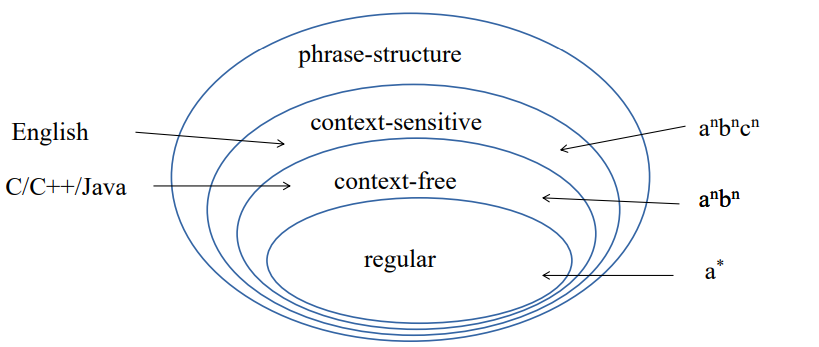
\includegraphics[width = 0.7\textwidth]{Images/ChomskyHierarchy.PNG}
    \caption{Chomsky Hierarchy}
    \label{fig:ChomskyHierarchy}
\end{figure}
\subsubsection{Turing Machines}
Context-sensitive and phrase-structure languages can be recognised by Turing machines. A Turing machine is basically an Non-Deterministic Finite Automaton with two sided tape, where more tapes do not increase the power. The Turing machine can compute "everything" that is computable with discrete states.
\subsection{Summary}
\begin{itemize}
    \item RegExp are truly useful in programming
    \item  Formal languages and grammars are truly useful to understand what computers can do
    \item RegExp, DFAs, NFAs & regular grammars all exactly correspond with regular languages
    \item Context-free grammars exactly correspond with Non-Deterministic Pushdown Automata
    \item Formal Languages form the Chomsky Hierarchy
\end{itemize}
